We compare the estimators at $n=10$, where every quantity can be computed exactly. The \emph{clustered} target is an equal mixture of four product distributions around random centres, each bit flipped with probability $0.1$. This target is smooth in Hamming distance. The \emph{checksum} target is the same mixture conditioned on even parity, which is a hard constraint that Hamming smoothing violates. For each target we draw $m\in\{30,100,300,1000\}$ samples over $10$ seeds.

The estimators are:
\begin{itemize}
\item the empirical distribution;
\item add-$\alpha$ (uniform pseudo-counts);
\item the heat / Aitchison--Aitken kernel;
\item the Tikhonov filter~\eqref{eq:p2};
\item penalised maximum likelihood~\eqref{eq:p1};
\item the learned positive isotropic filter of \cref{sec:filters} (LOO-EM), which has no hyperparameter.
\end{itemize}
To compare like with like, add-$\alpha$, heat and Tikhonov are tuned by the same criterion the learned filter optimises: full-data leave-one-out log-likelihood. Their grids include zero smoothing ($\alpha=0$, $\theta=0$, $\mu=0$). Zero smoothing is in fact never selected, and neither is the learned filter's identity endpoint $w_0=1$: without repeated strings both have leave-one-out likelihood $-\infty$. P1 has no closed-form leave-one-out score. Rather than refitting it $m$ times, we tune it on a $20\%$ validation split with the quadratic score $\|q\|_2^2-\frac{2}{|V|}\sum_{x\in V}q(x)$, a proper scoring rule~\cite{gneiting2007scoring}, and then refit on all $m$ samples. \Cref{tab:gen} and \cref{fig:gen} report the total-variation distance to the truth. Since all estimators see the same samples in each seed, we also report paired differences.

\begin{table}[t]
\centering
\caption{Total variation to the true distribution at $n=10$, given as mean (standard error $\times10^3$) over 10 seeds. Last column: mean mass on odd-parity strings for the checksum target at $m=100$, and the fraction of runs with $\mathrm{KL}(p\,\|\,q)<\infty$ for the clustered target at $m=1000$. Bold marks the best mean in each column.}\label{tab:gen}
\footnotesize
\setlength{\tabcolsep}{3pt}
\begin{tabular}{lccccccccc}
\toprule
& \multicolumn{4}{c}{clustered} & \multicolumn{4}{c}{checksum} & \\
\cmidrule(lr){2-5}\cmidrule(lr){6-9}
estimator & $m{=}30$ & $100$ & $300$ & $1000$ & $30$ & $100$ & $300$ & $1000$ & invalid / KL fin.\\
\midrule
empirical & .611(10) & .421(12) & .310(5) & .185(4) & .502(16) & .344(12) & .239(6) & \textbf{.136}(4) & 0 / 0.0\\
add-$\alpha$ & .562(12) & .439(17) & .327(3) & .183(3) & .553(8) & .364(10) & .275(14) & .162(5) & .115 / 1.0\\
heat (A--A) & \textbf{.403}(14) & \textbf{.284}(10) & \textbf{.238}(4) & \textbf{.164}(4) & .585(6) & .460(12) & .342(6) & .207(22) & .326 / 1.0\\
Tikhonov (P2) & .417(16) & .290(9) & .246(6) & .168(4) & .552(10) & .426(12) & .331(10) & .206(8) & .270 / 1.0\\
pen.\ MLE (P1) & .546(16) & .421(11) & .333(12) & .188(4) & .580(23) & .353(12) & .256(9) & .147(5) & .001 / 0.0\\
learned isotropic & .417(14) & .288(10) & \textbf{.238}(4) & .168(4) & \textbf{.382}(12) & \textbf{.269}(11) & \textbf{.210}(8) & \textbf{.136}(3) & 0 / 0.9\\
\bottomrule
\end{tabular}
\end{table}

\begin{figure}[t]
\centering
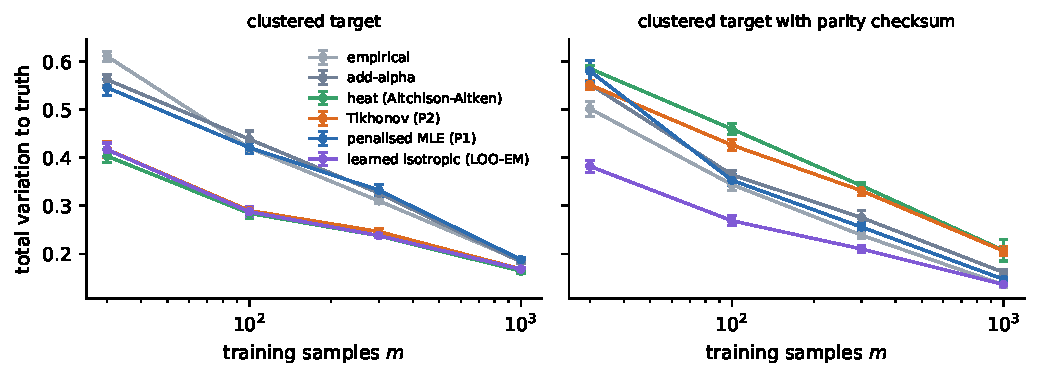
\includegraphics[width=\linewidth]{figures/fig_generalisation.pdf}
\caption{Total variation to the truth at $n=10$ (mean $\pm$ s.e., 10 seeds). On the smooth target, heat, Tikhonov and the learned filter are close to each other and well below the empirical distribution, while P1 barely improves on it. On the checksum target, the Hamming smoothers lose to the empirical distribution, and only the learned isotropic filter improves on it.}\label{fig:gen}
\end{figure}

\paragraph{Smooth target.}
Heat, Tikhonov and the learned filter all beat the empirical distribution and add-$\alpha$ at every $m$. The gain is largest at small $m$: at $m=30$, TV drops from $0.61$ to $0.40$--$0.42$. Among the three, the one-parameter heat kernel is as good as or slightly better than the learned filter. The paired difference (learned minus heat) is $+0.014\pm0.004$ at $m=30$ and $+0.004\pm0.001$ at $m=1000$, and within two standard errors of zero at $m=100$ and $300$. Against Tikhonov, the learned filter is within one standard error at $m=30$, $100$ and $1000$, and better by $0.008\pm0.003$ at $m=300$. On a target that really is Hamming-smooth, then, learning all $n+1$ shell weights buys nothing over tuning a single bandwidth by the same criterion, and costs a little variance at small $m$.

\paragraph{Penalised likelihood barely smooths here.}
P1 barely improves on the empirical distribution, and it has infinite KL in every run. This is consistent with \cref{prop:support}. In the runs we inspected ($m=100$ and $1000$), the support of the P1 optimum stays exactly equal to the set of distinct observed strings across the whole useful range of $\mu$. So in this regime P1 only \emph{reweights} the observed strings: it compresses the frequent ones and lifts the rare ones, but it does not move mass onto unseen strings, which is where most of the error lies. This is a property of the regime, not a general law. With few distinct strings and strong smoothing, P1 does spread mass (\cref{sec:exp-small}; the $n=1$ example in \cref{sec:p1}). Here larger $\mu$ only hurts, and validation drives $\mu\to0$ at large $m$. The cause is the likelihood term, which rewards mass on the data and gives no direct reward for mass elsewhere. The $\ell_2$ data term of P2 has no such effect.

\paragraph{The checksum counterexample.}
On the parity-constrained target, the Hamming smoothers lose to the empirical distribution at every $m$. Part of this is structural. Any heat kernel with $\theta>0$ leaks the mass $\Pr[\text{odd number of flips}]=\tfrac12\bigl(1-(1-2\theta)^{n}\bigr)$, which is already $4.8\%$ at the smallest positive grid value $\theta=0.005$. Leave-one-out selection makes this worse, not better: it favours $\theta\approx0.1$ at $m=30$, and heat and Tikhonov then put $27$--$45\%$ of their mass on invalid strings at $m\le100$.

The learned isotropic filter is the exception. It places \emph{exactly zero} mass on invalid strings. It beats heat and Tikhonov by $0.07$--$0.20$ in TV in every seed at every $m$, and it beats the empirical distribution in every seed for $m\le300$, tying it at $m=1000$. Its weights show why. For one seed at $m=100$, EM returns $w_0=0.74$, $w_2=0.26$ and $w_d=0$ otherwise. All pairwise distances within the data are even, so the leave-one-out likelihood puts all weight on even shells, and ``flip exactly two bits'' preserves parity. Isotropic does not mean Hamming-local. The positive isotropic class of \cref{thm:isotropic} is rich enough to express some hard constraints, while remaining exactly samplable in $O(n)$. The price is that zero weight on some shells can leave valid strings with zero mass, so its KL is not always finite at small $m$.
